\documentclass[a4paper,14pt]{extarticle}
\usepackage{../../tex-shared/report-layout}

\renewcommand{\mylabnumber}{1}
\renewcommand{\mylabtitle}{Исследование базовых функций языка Лисп}
\renewcommand{\mysubject}{Методы и средства искусственного интеллекта}
\renewcommand{\mylecturer}{Сметанина Т.И.}

\begin{document}
\begin{titlepage}
    
    \thispagestyle{empty}
    
    \begin{center}
        
        Министерство науки и Высшего образования Российской Федерации \\
        Севастопольский государственный университет \\
        Кафедра ИС
        
        \vfill

        Отчет \\
        по лабораторной работе №\mylabnumber \\
        \enquote{\mylabtitle} \\
        по дисциплине \\
        \enquote{\MakeTextUppercase{\mysubject}}

    \end{center}

    \vspace{1cm}

    \noindent\hspace{7.5cm} Выполнил студент группы ИС/б-17-2-о \\
    \null\hspace{7.5cm} Горбенко К. Н. \\
    \null\hspace{7.5cm} Проверил \\
    \null\hspace{7.5cm} \mylecturer

    \vfill

    \begin{center}
        Севастополь \\
        \the\year{}
    \end{center}

\end{titlepage}

\section{Цель работы}
Изучение технологии подготовки и выполнения Лисп-программ в выбранной
интегрированной среде, исследование свойств базовых функций обработки списков, а
также способов описания и вызова нерекурсивных функций в языке программирования
Лисп.

\section{Задание на работу}
\begin{enumerate}
    \item Изучить среду программирования на языке Лисп по методическим
          указаниям.
    \item Определить на языке Лисп функцию в соответствии с вариантом задания.
          Определение выполнить различными способами, применяя базовые функции
          обработки списков (см. п. 1.2.2) и дополнительные функции (см. п.1.2.3).
    \item Создать в среде программирования Лисп-проект в соответствии с
          методическими указаниями, содержащий подготовленные определения функций
          и вызовы функций при различных значениях аргументов, в том числе и не
          допустимых.
    \item Выполнить отладку проекта.
    \item Зафиксировать результаты выполнения функций и ошибки, возникающие при
          недопустимых значениях аргументов (в виде экранных копий).
    \item Объяснить результаты и локализовать вызовы функции, порождающие ошибки.
    \item Исследовать отдельно каждую базовую и дополнительную функцию, входящую
          в определения функций, выполненных в п.1.4.3. Привести примеры правильных и
          неправильных вызовов.
\end{enumerate}

Задание по варианту: описать на языке Лисп функцию \code{f(x y z)} от трёх аргументов,
которая формирует из своих аргументов список и выполняет его обработку следующим
образом.

Проверить, является ли хотя бы один из элементов списка списком. Если является,
то вернуть этот список без первого элемента, иначе поменять местами первый и
второй элементы исходного списка.

\section{Ход работы}
\subsection{Определения функций}
Определим функции в соответствии с вариантом. Функция \code{f1} определена с
помощью базовых функций языка \code{LISP}. 

Использованы функции \code{car} (возвращает первый элемент списка), \code{cdr}
(возвращает второй элемент списка), \code{cons} (составляет список). Для
ветвления использовалась функция \code{if} (аналог тернарного оператора).

Функция \code{let} используется для создания локальных переменных и области их
видимости.
\begin{lstlisting}
(defun f1 (x y z)
  (let ((items (cons x (cons y (cons z nil)))))
    (if (some #'listp items)
      (cdr items)
      (cons
        (car (cdr items))
        (cons
          (car items)
          (cdr (cdr items))
        )
      )
    )
  )
)
\end{lstlisting}

Функция \code{f2} определена с помощью дополнительных функций. Кроме функций,
перечисленных выше, были использованы: \code{list} -- функция для компоновки
списков, \code{some} -- возвращает признак того, выполняется ли данный предикат
хотя бы для одного элемента списка, \code{rest} -- возвращает все элементы
списка кроме первого, \code{first}, \code{second}, \code{third} -- возвращают
соответствующий (по счету) элемент списка.
\begin{lstlisting}
(defun f2 (x y z)
  (let ((items (list x y z)))
    (if (some #'listp items)
      (rest items)
      (list (second items) (first items) (third items))
    )
  )
)
\end{lstlisting}

\subsection{Выполним программу}
Передавая этим функциям одинаковые параметры, проверим их работу.
\begin{lstlisting}
(print (f1 1 2 (list 1 2 3)))
(print (f1 1 2 3))
(print (f2 1 2 (list 1 2 3)))
(print (f2 1 2 3))
\end{lstlisting}

Результат работы программы изображен на рисунке \ref{fig:result}:
\begin{figure}[H]
    \centering
    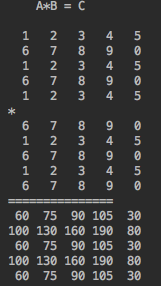
\includegraphics[width=.8\linewidth]{result}
    \caption{Результат работы программмы}
    \label{fig:result}
\end{figure}

Из результатов работы программы видно, что обе функции работают одинаково верно.

\section*{Выводы}
В ходе лабораторной работы были использованы базовые функции языка \code{LISP} и 
способы описания функций. Для описания функций используются функция \code{defun}.

Изучены функции:
\begin{itemize}
    \item \code{car} -- возвращает первый элемент списка;
    \item \code{cdr} -- возвращает второй элемент списка;
    \item \code{cons} -- составляет список;
    \item \code{if} -- используется для организации ветвления (аналог тернарного оператора);
    \item \code{let} -- используется для создания локальных переменных и области их видимости;
    \item \code{list} -- создает список из параметров;
    \item \code{some} -- возвращает признак того, выполняется ли данный предикат
          хотя бы для одного элемента списка;
    \item \code{rest} -- возвращает все элементы списка кроме первого;
\end{itemize}

\end{document}